\subsubsection{Shorter Paths}
\label{sec:sphinx:shorterpaths}

SPHINX packets define a maximum path length $r$, meaning $r$ intermediate mix nodes and one destination. They also allow the use of shorter paths of length $v$ with $0 \le v < r$. Despite these packets being the same size and being indistinguishable from packets with maximum path length due to their construction, it not advisable to use shorter paths since they introduce observable patterns that deviate from normal usage. By default, HOPR nodes use a path length of three and refuse to process packets with greater path lengths. 

Creating a header for shorter paths require less routing information, and thus leaves empty space in the end of $\beta$, which is filled as suggested by \cite{sphinxpaperfix} with \textit{random} data. This is necessary because the very last node, $Z$, is otherwise able to determine the path length.

\begin{figure}[H]
    \centering
    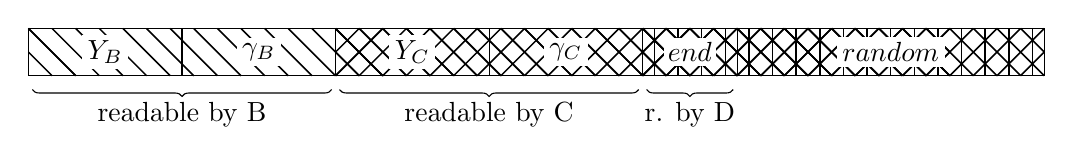
\begin{tikzpicture}
        \def\one{0.6}
        \def\scale{0.9}
        \def\nodeWidth{1.95}
        \def\endWidth{1.2}
        \def\width{3*2*\nodeWidth+\endWidth}
        \foreach \i\name in{0/B,1/C,2/D,3/Z} {
                \begin{scope}[shift={(\i*\nodeWidth*2,0)}]
                    \ifnum\i=0
                        \def\a{11.7}
                        \def\diff{11.1}
                    \fi

                    \ifnum\i=1
                        \def\a{7.8}
                        \def\diff{7.2}
                    \fi

                    \ifnum\i=2
                        \def\a{5.1}
                        \def\diff{4.5}
                    \fi

                    \def\b{\one}
                    \def\lw{0.2}

                    \ifnum\i<3
                        \foreach \x [count=\i] in{0,0.3,0.6,...,\b}{
                                \draw [line width=\lw mm](\x,0)--(0,\x) (\a-\b+\x,\b)--(\a,\x);
                            }
                        \foreach \x [count=\i] in{0,0.3,0.6,...,\diff}{
                                \draw [line width=\lw mm](\x+\b,0)--(\x,\b);
                            }

                        \ifnum\i>0
                            \foreach \x [count=\i] in{0,0.3,0.6,...,\b}{
                                    \draw [line width=\lw mm](0,\x)--(\b-\x,\b) (\a-\b+\x,0)--(\a,\b-\x);
                                }
                            \foreach \x [count=\i] in{0,0.3,0.6,...,\diff}{
                                    \draw [line width=\lw mm](\x,0)--(\b+\x,\b);
                                }
                        \fi

                        \ifnum\i>1
                            \foreach \x [count=\i] in{0.15,0.45,...,\a}{
                                    \draw [line width=\lw mm](\x,0)--(\x,\b);
                                }
                        \fi
                    \fi
                \end{scope}
                \ifnum\i=3
                    \draw (\i*2*\nodeWidth-2*\nodeWidth+\endWidth,0) rectangle (\i*2*\nodeWidth+\endWidth,\one) node [midway,fill=white,inner sep=2pt] {$random$};
                \else
                    \ifnum\i<2
                        \draw [color=white] (\i*2*\nodeWidth,0) rectangle (\i*2*\nodeWidth+\nodeWidth,\one) node [midway,color=black,fill=white,inner sep=2pt] {$Y_{\name}$};
                        \draw (\i*2*\nodeWidth,0) -- (\i*2*\nodeWidth,\one);
                        \draw [color=white] (\i*2*\nodeWidth+\nodeWidth,0) rectangle (\i*2*\nodeWidth+2*\nodeWidth,\one) node [midway,color=black,fill=white,inner sep=2pt] {$\gamma_{\name}$};
                        \draw (\i*2*\nodeWidth+\nodeWidth,0) -- (\i*2*\nodeWidth+\nodeWidth,\one);

                        \draw[decoration={brace,raise=5pt,mirror},decorate] (\nodeWidth*2*\i+0.05,0) -- (\nodeWidth*2*\i+\nodeWidth*2-0.05,0) node[midway,below=6pt] {readable by \name};
                    \else
                        \draw [color=white] (\i*2*\nodeWidth,0) rectangle (\i*2*\nodeWidth+\endWidth,\one) node [midway,color=black,fill=white,inner sep=1.5pt] {$end$};

                        \draw (\i*2*\nodeWidth,0) -- (\i*2*\nodeWidth,\one);
                        \draw (\i*2*\nodeWidth+\endWidth,0) -- (\i*2*\nodeWidth+\endWidth,\one);

                        \draw[decoration={brace,raise=5pt,mirror},decorate] (\i*2*\nodeWidth+0.05,0) -- (\i*2*\nodeWidth+\endWidth-0.05,0) node[midway,below=6pt] {r. by \name};
                    \fi
                \fi
            }

        \draw (0,0) rectangle (\width,\one);
    \end{tikzpicture}
    \caption{Node $A$ has created routing information for $B,C$ and the final recipient $D$, filling the empty part of $\beta$ with random data.}
\end{figure}

By applying the transformations seen in section \ref{sec:sphinx:shifting} through the mixnet nodes, all blindings got removed, hence the plaintext of $\beta$ becomes visible and the node is able to decide which parts of $\beta$ were not used.

\begin{figure}[H]
    \centering
    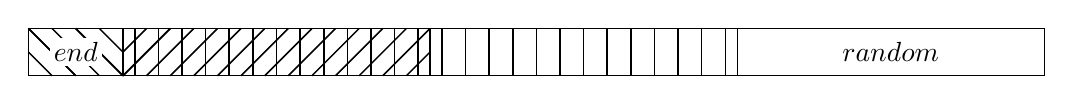
\begin{tikzpicture}
        \def\one{0.6}
        \def\scale{0.9}
        \def\nodeWidth{1.95}
        \def\endWidth{1.2}
        \def\width{3*2*\nodeWidth+\endWidth}
        \foreach \i\name in{0/B,1/C,2/D,3/Z} {
                \ifnum\i=2
                    \def\a{7.8}
                    \def\diff{7.2}
                \fi

                \ifnum\i=1
                    \def\a{3.9}
                    \def\diff{3.3}
                \fi

                \ifnum\i=0
                    \def\a{\endWidth}
                    \def\diff{0.6}
                \fi


                \def\b{0.6}
                \def\lw{0.2}

                \ifnum\i=0
                    \foreach \x [count=\i] in{0,0.3,0.6,...,\b}{
                            \draw [line width=\lw mm](\x,0)--(0,\x) (\a-\b+\x,\b)--(\a,\x);
                        }
                    \foreach \x [count=\i] in{0,0.3,0.6,...,\diff}{
                            \draw [line width=\lw mm](\x+\b,0)--(\x,\b);
                        }

                \fi
                \begin{scope}[shift={(\endWidth,0)}]
                    \ifnum\i=1
                        \foreach \x [count=\i] in{0,0.3,0.6,...,\b}{
                                \draw [line width=\lw mm](0,\x)--(\b-\x,\b) (\a-\b+\x,0)--(\a,\b-\x);
                            }
                        \foreach \x [count=\i] in{0,0.3,0.6,...,\diff}{
                                \draw [line width=\lw mm](\x,0)--(\b+\x,\b);
                            }
                    \fi

                    \ifnum\i=2
                        \foreach \x [count=\i] in{0.15,0.45,...,\a}{
                                \draw [line width=\lw mm](\x,0)--(\x,\b);
                            }
                    \fi
                \end{scope}

                \ifnum\i=3
                    \draw (\i*2*\nodeWidth-2*\nodeWidth+\endWidth,0) rectangle (\i*2*\nodeWidth+\endWidth,\one) node [midway] {$random$};
                \else
                    \ifnum\i>0
                        \draw (\i*2*\nodeWidth+\endWidth,0) -- (\i*2*\nodeWidth+\endWidth,\one);
                    \else
                        \draw [color=white] (\i*2*\nodeWidth,0) rectangle (\i*2*\nodeWidth+\endWidth,\one) node [midway,color=black,fill=white,inner sep=1.5pt] {$end$};
                        \draw (\endWidth,0) -- (\endWidth,\one);
                    \fi
                \fi
            }

        \draw (0,0) rectangle (\width,\one);
    \end{tikzpicture}
    \caption{Node $D$ receives a packet which was relayed by two intermediate nodes.}
\end{figure}
